\documentclass[../../../../main.tex]{subfiles}
\begin{document}

\begin{flushright}
\footnotesize\textit{【自動文字起こし・要確認】}
\end{flushright}

\begin{proof}[解]
(1) $S$ のベクトル $\vec{a}, \vec{b}$ のなす角を $\theta$ とすると ($0 \le \theta \le \pi$), 条件から
\[
2 \frac{|\vec{a}|}{|\vec{b}|} \cos\theta \in \mathbb{Z}
\]
又、$\vec{a}, \vec{b}$ を逆にした
\[
2 \frac{|\vec{b}|}{|\vec{a}|} \cos\theta \in \mathbb{Z}
\]
も成り立ち、したがって、辺々かけあわせて
\[
4 \cos^2\theta \in \mathbb{Z} \quad \cdots \text{①}
\]
$0 \le \cos^2\theta \le 1$ だから、①がみたされるのは
\[
4 \cos^2\theta = 0, 1, 2, 3, 4
\]
\[
\iff \cos^2\theta = 0, \frac{1}{4}, \frac{1}{2}, \frac{3}{4}, 1
\]
\[
\iff \cos\theta = 0, \pm \frac{1}{2}, \pm \frac{1}{\sqrt{2}}, \pm \frac{\sqrt{3}}{2}, \pm 1
\]
\[
\iff \theta = 0, \frac{\pi}{6}, \frac{\pi}{4}, \frac{\pi}{3}, \frac{\pi}{2}, \frac{2}{3}\pi, \frac{3}{4}\pi, \frac{5}{6}\pi, \pi
\]
より題意は示された.

\medskip
(2) 角が $0$ の時. $2 \frac{|\vec{a}|}{|\vec{b}|}, 2 \frac{|\vec{b}|}{|\vec{a}|} \in \mathbb{Z}$ から,
\[
2 \frac{|\vec{a}|}{|\vec{b}|} = k, \quad 2 \frac{|\vec{b}|}{|\vec{a}|} = m \quad (k, m \in \mathbb{N})
\]
とおける. 辺々かけあわせて $4 = km$ より $(k, m) = (1, 4), (2, 2), (4, 1)$ だが、このうち $|\vec{a}| = |\vec{b}| \iff k = 2 = m$ を満たすのは $k=1, 2$ の時で
\[
|\vec{a}| : |\vec{b}| = 1 : 1, \quad 1 : 2
\]
・角が $\pi/6$ の時, 同様に $k, m \in \mathbb{N}$ として
\[
\sqrt{3} \frac{|\vec{a}|}{|\vec{b}|} = k, \quad \sqrt{3} \frac{|\vec{b}|}{|\vec{a}|} = m
\]
辺々かけて $3 = km$ より $(k, m) = (1, 3), (3, 1)$. これらは $|\vec{a}| : |\vec{b}| = k : \sqrt{3} = \sqrt{3} : m$ をみたすから、2ベクトルの比は $1 : \sqrt{3}$.

・角が $\pi/3$ の時, $\frac{|\vec{a}|}{|\vec{b}|}, \frac{|\vec{b}|}{|\vec{a}|} \in \mathbb{Z}$ から ベクトルの比は $1 : 1$.

\medskip
(3) まず, $\vec{a} = \begin{pmatrix} 1 \\ 0 \end{pmatrix}, \vec{b} = |\vec{b}| \begin{pmatrix} \cos \pi/6 \\ \sin \pi/6 \end{pmatrix}$ とおける. なす角が $120^\circ, 150^\circ$ の時の2ベクトルの比は (2)の $60^\circ, 30^\circ$ の場合に等しく, $90^\circ$ の時は鏡であることから、下図のようにとればこれらは集合 $S$ になる. (ただし片方のベクトルのなす角 $30^\circ$)

\begin{center}
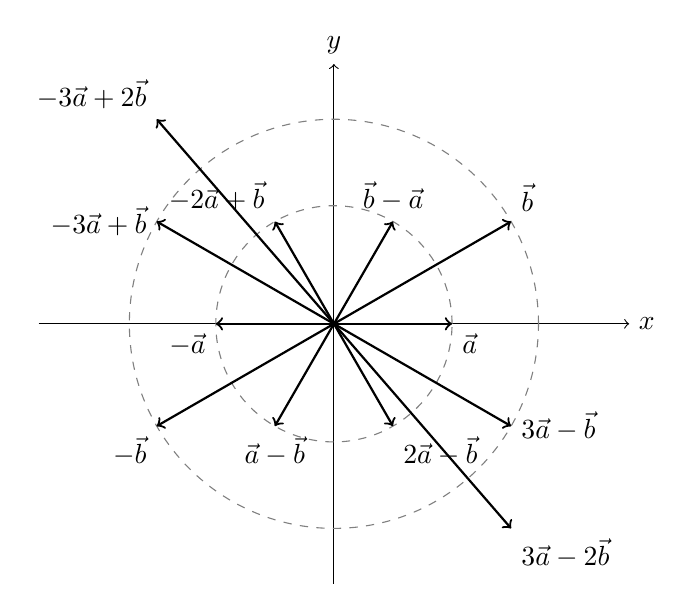
\begin{tikzpicture}[scale=1.5]
  \draw[->] (-2.5,0) -- (2.5,0) node[right] {$x$};
  \draw[->] (0,-2.2) -- (0,2.2) node[above] {$y$};
  \draw[dashed, gray] (0,0) circle (1);
  \draw[dashed, gray] (0,0) circle (1.732);
  
  % Rays / Vectors
  \draw[->, thick] (0,0) -- (1,0) node[below right] {$\vec{a}$};
  \draw[->, thick] (0,0) -- (1.5, 0.866) node[above right] {$\vec{b}$};
  \draw[->, thick] (0,0) -- (0.5, 0.866) node[above] {$\vec{b}-\vec{a}$};
  \draw[->, thick] (0,0) -- (-1.5, 1.732) node[above left] {$-3\vec{a}+2\vec{b}$};
  \draw[->, thick] (0,0) -- (-0.5, 0.866) node[above left] {$-2\vec{a}+\vec{b}$};
  \draw[->, thick] (0,0) -- (-1.5, 0.866) node[left] {$-3\vec{a}+\vec{b}$};
  \draw[->, thick] (0,0) -- (-1,0) node[below left] {$-\vec{a}$};
  \draw[->, thick] (0,0) -- (-1.5, -0.866) node[below left] {$-\vec{b}$};
  \draw[->, thick] (0,0) -- (-0.5, -0.866) node[below] {$\vec{a}-\vec{b}$};
  \draw[->, thick] (0,0) -- (1.5, -1.732) node[below right] {$3\vec{a}-2\vec{b}$};
  \draw[->, thick] (0,0) -- (0.5, -0.866) node[below right] {$2\vec{a}-\vec{b}$};
  \draw[->, thick] (0,0) -- (1.5, -0.866) node[right] {$3\vec{a}-\vec{b}$};
\end{tikzpicture}
\end{center}

これらを $\vec{a}, \vec{b}$ で表すと、$\vec{a}, \vec{b}$ から反時計回りに順に
\[
\vec{a}, \, \vec{b}, \, \vec{b}-\vec{a}, \, -3\vec{a}+2\vec{b}, \, -2\vec{a}+\vec{b}, \, -3\vec{a}+\vec{b}, \, -\vec{a}, \, -\vec{b}, \, \vec{a}-\vec{b}, \, 3\vec{a}-2\vec{b}, \, 2\vec{a}-\vec{b}, \, 3\vec{a}-\vec{b}
\]
\end{proof}

\newpage

\end{document}
